\documentclass[11pt]{article}
\usepackage[a4paper,margin=1in]{geometry}
\usepackage{amsmath,amssymb,amsthm,mathtools}
\usepackage{booktabs}
\usepackage{enumitem}
\usepackage{graphicx}
\usepackage{microtype}
\usepackage{hyperref}
\usepackage[nameinlink,capitalise]{cleveref}
\usepackage[numbers,sort&compress]{natbib}

\newtheorem{theorem}{Theorem}[section]
\newtheorem{proposition}[theorem]{Proposition}
\newtheorem{corollary}[theorem]{Corollary}
\theoremstyle{definition}
\newtheorem{definition}[theorem]{Definition}
\theoremstyle{remark}
\newtheorem{remark}[theorem]{Remark}
\newcommand{\mathsfclosed}{\mathsf{closed}}
\newcommand{\mathsfopen}{\mathsf{open}}
\newcommand{\mathsfred}{\mathsf{red}}
\newcommand{\norm}[1]{\left\lVert#1\right\rVert}

\title{A Hundred-Layer Audit of Prime Dynamics\\
\large Exact Theorems, Negative Routes, and the Minimal Stage-A/A5 Frontier}
\author{Liang Wang}
\date{July 2026}

\begin{document}
\maketitle

\begin{abstract}
We audit the first ninety-nine RH layers of the quadratic prime-dynamics
program before selecting the post-centennial route.  The repository contains
ninety-nine consecutive paper directories, each with manuscript source and a
paper PDF; seventy have machine-readable summary archives.  We classify the
layers into nine phases, distinguish exact theorems from frozen finite
validation, conditional composition, negative branch results, and genuinely
open all-level gates, and hash every available README, manuscript, and summary
input.

We extend the earlier route-synthesis method to a status-aware completion
frontier theorem.  In a monotone AND/OR dependency formula, a closed leaf
contributes no proof debt, an open leaf contributes its singleton, a red leaf
contributes no viable branch, OR takes antichain union, and AND takes the
antichain of Cartesian unions.  This rule permits conservative substitution
of a decomposed subroute without promoting finite validation to an all-level
theorem.

Applied after RH-99, unconditional Stage A has exactly three
inclusion-minimal completion bundles.  The fallback is the singleton
\[
 \{L\},
\]
the RH-75 all-level full-block law.  The packet alternatives are
\[
 \{Q,G,H_{\rm stop},O\},
 \qquad
 \{Q,G,H_{\rm tube},O\},
\]
where $Q$ is a uniform gap-aware quotient law, $G$ a structured packet action
for the normalized memory Gramian, $O$ the prefix/normalization/observability
bridge, and the two $H$ gates are stopped-hybrid or finite differential
horizon propagation.

RH-94--RH-99 materially revise the preference between these alternatives.
Source seeding, reduced cross factorization, local weak-mode quotienting, and
exact nonlinear hybrid budgets are positive.  Binary64 moment-only closure,
aggressive quotient cutoffs, universal unit propagation, and the current
first-order differential tube are negative.  Five fine-scale Ritz gaps remain
uncertified and available differential constants are unusably large.
Therefore the preferred packet route is
$Q\wedge G\wedge H_{\rm stop}\wedge O$; the smooth tube is retained as a
research alternative, not treated as closed.

Every Stage-A bundle still needs three independent Stage-A5 gates: an actual
moving-cloud Riesz projection, its coefficient bridge, and a uniform
trace-class complement.  Canonical scattering completion, self-adjoint
realization, intrinsic $T\log T$ counting, a prime-power trace formula, and
zeta-zero identification remain downstream.

The selected next sequence is RH-101 on finite-memory packet Gram action,
RH-102 on a stopped quotient clock, and RH-103 on the prefix and observability
ledger.  No unconditional Stage A, Hilbert--Polya operator, zero
identification, or Riemann Hypothesis result is claimed.
\end{abstract}

\noindent\textbf{Keywords:} research roadmap; dependency antichain; validated
numerics; projected-cross Ritz method; moving-cloud determinant; claim audit.

\medskip
\noindent\textbf{MSC 2020:} 37C30; 47A75; 65G20; 11M26.

\section{Purpose and audit discipline}

The RH sequence began by asking whether the numerical and symbolic-dynamical
claims surrounding the prime/logistic construction could be reformulated
without placing an unproved admissibility hypothesis inside every conclusion.
It then moved through regularized cycle determinants, small-noise spectral
limits, critical branch returns, validated contour methods, continuum
identification, directional Hardy energies, Stage-A composition, moving-cloud
relative determinants, and finally recursive low-rank packet dynamics.

After ninety-nine layers, simple continuation is no longer the right
planning method.  Several branches have become exact, several have failed for
specific reasons, and several finite certificates remain far from all-level
theorems.  A centennial review must preserve those distinctions.

We use five statuses.
\begin{enumerate}[leftmargin=2em]
\item \emph{Exact}: a finite-dimensional or analytic theorem proved in the
manuscript's stated scope.
\item \emph{Frozen green}: an outward-rounded or exact-stored certificate for
named finite arrays and scales.
\item \emph{Conditional green}: a rigorous implication whose premise is an
open all-level estimate.
\item \emph{Red branch}: a precise proposed mechanism or shortcut rejected by
a theorem or counterexample.
\item \emph{Open}: a primitive all-level gate not supplied by the earlier
statuses.
\end{enumerate}
A red branch is not a no-go theorem for the whole program.  Conversely,
ninety-nine successful finite computations do not close one open uniform
leaf.

\section{Ninety-nine-layer inventory}
\label{sec:inventory}

The automated inventory finds:
\begin{align*}
  &99\ \text{README files},\qquad
    99\ \text{main TeX files},\\
  &99\ \text{paper-PDF directories},\qquad
    70\ \text{summary archives}.
\end{align*}
Early layers predate the common summary schema, but all manuscript and README
inputs are hashed in the RH-100 archive.

\begin{table}[t]
\centering
\caption{Nine phases of the RH-1--RH-99 sequence.}
\label{tab:phases}
\begin{tabular}{@{}rllr@{}}
\toprule
layers & count & main theme & summaries\\
\midrule
1--12  & 12 & symbolic reformulation, cycles, small-noise limits & 0\\
13--23 & 11 & parity boundary layers and critical branches & 0\\
24--34 & 11 & contour, Rouch\'e, resolvent, Grushin validation & 5\\
35--49 & 15 & physical counting, continuum/Riesz identification & 15\\
50--61 & 12 & Hardy energies, Stein metrics, phase/horizon laws & 12\\
62--71 & 10 & Krylov/covariance closure and upstream validation & 10\\
72--81 & 10 & finite Stage A and moving-cloud A5 frontier & 10\\
82--91 & 10 & rank clocks, packets, Ritz and Schur certificates & 10\\
92--99 & 8  & recursive horizons, quotient and propagation barriers & 8\\
\bottomrule
\end{tabular}
\end{table}

\subsection{Layers 1--34: from symbolic reformulation to validated resolvents}

RH-1 separates the published Paper-1 structural claims from the topological
admissibility hypothesis rather than silently using the hypothesis as a
theorem.  RH-2--RH-12 build exact prime-kneading finite words, parity-resolved
spectra, renormalized response, noncommuting small-noise/long-cycle limits,
time-ordered traces, and regularized determinants.  The key lesson is already
visible at RH-10: long-cycle and small-noise limits need a logarithmic horizon
and cannot be interchanged without proof.

RH-13--RH-23 resolve parity boundary layers and critical-return channels.
The two-branch factorization and dark-mode algebra are exact, while proposed
single-sibling and phase shortcuts are marked conditional or red.  The
complement cannot be treated as a negligible scalar remainder.

RH-24--RH-34 convert root-count heuristics into contour, Rouch\'e,
primal-dual, rational Arnoldi, deflated complement, sparse Grushin, and inertia
certificates.  These papers establish a durable methodology: floating
algorithms select candidates; exact-stored interval arithmetic certifies the
named matrices and residual inequalities.  They do not promote the binary64
assembly pipeline to a continuum theorem.

\subsection{Layers 35--71: intrinsic identification and directional tails}

RH-35--RH-49 replace coordinate-dependent eigenvectors by physical packet
counts, nested-grid limits, adaptive cutoffs, and weighted Riesz projectors.
The gauge-invariant object
\[
 A\Pi(A;\Gamma)
\]
provides the correct finite-to-continuum branch quantity.  Intrinsic
identification is reduced to directional complement resolvent actions, not
global operator norm.

RH-50 gives a decisive positive/negative pair.  Directional
Hilbert--Schmidt Hardy energies admit exact Laurent and Stein bounds, while a
noise-uniform fixed-step global contraction is impossible because the
deterministic complement is isometric.  RH-51--RH-61 explore cyclic ranks,
residue transfer, cutoffs, mixed Haar channels, Schur metrics, phase-aware
tails, and horizon scaling.  Several finite fusions work; direction-free
uniform horizon estimates carry forbidden scale powers.

RH-62--RH-71 develop nested Krylov residuals, weighted terminal errors,
physical covariance blocks, adaptive certificate portfolios, and finally a
frozen production block Hardy certificate.  By RH-70, all terminal tail
calculations are outward-rounded and green.  The remaining validation wall
has moved upstream to assembly, deflation, and family-uniform transfer.  RH-71
records this change of location rather than declaring Stage A complete.

\subsection{Layers 72--81: finite Stage A and moving-cloud A5}

RH-72--RH-74 close the complete five-scale folded-Gaussian assembly,
rank-two deflation, and upstream Hardy chain.  RH-75 states an explicit
all-level log-square full-block law; it is a sufficient theorem template but
is validated only at the anchors.  RH-76 rejects single-arc phase compression.
RH-77 finds exceptional postblock rank-two/rank-four compression, and RH-78
proves that either the full-block or effective-rank corridor would close
Stage A conditionally with zero Hardy power.

RH-79 reaches two-step trace norm and shrinking-disk determinants.  RH-80
proves that fixed scalar pole cancellation fails outside the cloud circle and
replaces it with an exact moving-cloud relative factorization
\citep{WangCloud2026}.  RH-81's review identifies three independent A5 gates:
an actual cloud Riesz projection, a coefficient bridge, and a uniform
trace-class complement \citep{WangRouteReview2026}.

\subsection{Layers 82--91: packet reduction of the effective-rank wall}

The second ten-layer review begins with a half-log rank clock and progressively
weakens exact endpoint factorization to captured energy.  Strict-prefix and
trace-normalized late-memory packets reduce drift to small Rayleigh and Schur
objects.  Global norm contraction and point-packet contraction are rejected.
Rank-one complement Ritz correction and the Schur-secular sign theorem remove
the ambient reference packet from the finite one-step certificate.

RH-91 concludes that Stage A has two alternatives: prove the all-level
full-block law, or complete a packet bundle consisting of uniform late
contraction, reduced future control, and the prefix/observability bridge
\citep{WangPacketReview2026}.  At that point, however, each late block still
begins from an ambient leading packet.

\subsection{Layers 92--99: recursive packets and the propagation frontier}

RH-92 replaces rigid pointwise sub-quarter decay by a four-step product
budget.  RH-93 proves multi-direction recursive Ritz refresh and shows one
direction fails while two close every selected late block.  RH-94 moves the
only seed to time zero: the initial normalized Gram packet is exactly the
source right singular packet, and width four tracks every complete frozen
prefix \citep{WangSourceSeed2026}.

RH-95 removes the ambient cross SVD algebraically through reduced moments, but
discovers that binary64 moment-only closure is ill conditioned.  RH-96 proves
a gap-weighted weak-mode quotient theorem and safely drops exactly five weak
fourth modes at cutoff $10^{-8}$ \citep{WangWeakMode2026}.  Larger cutoffs
remain locally certified but fail cumulatively.

RH-97 solves finite accumulation exactly by nonlinear hybrid telescoping
\citep{WangHybrid2026}.  RH-98 proves the projector envelope but constructs a
strictly positive trace-one counterexample amplifying local tail loss by more
than forty-four; universal unit propagation is false
\citep{WangProjectorBarrier2026}.  RH-99 derives the correct two-gap
differential formula, yet five fine-scale output Ritz gaps are unavailable and
the first-order tube is unusable \citep{WangDifferential2026}.

\begin{figure}[t]
\centering
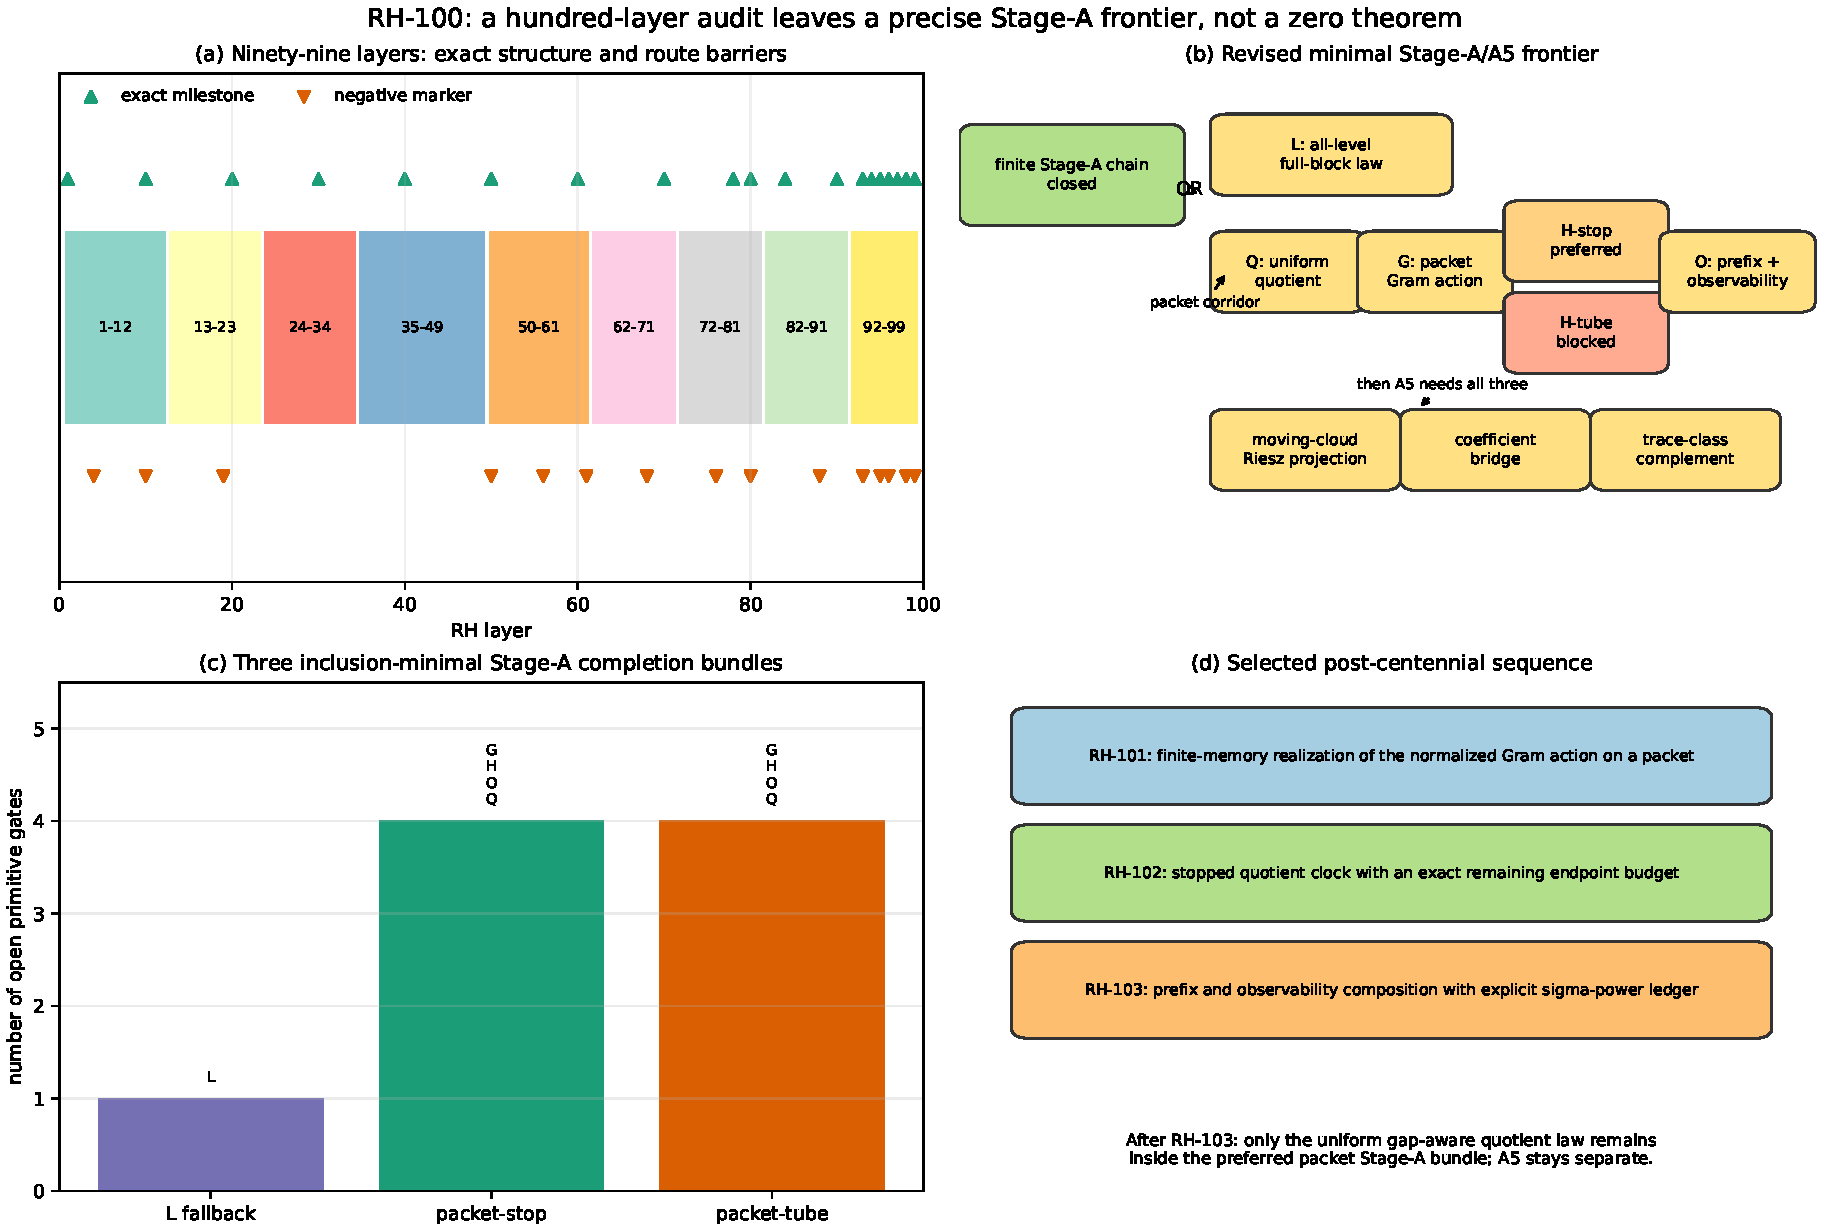
\includegraphics[width=\textwidth]{figures/hundred_layer_route_review.pdf}
\caption{Centennial inventory and revised frontier.  Exact milestones and red
branches coexist; the preferred packet route has four open primitive gates,
while the one-gate full-block corridor remains a fallback.}
\label{fig:review}
\end{figure}

\section{Status-aware completion frontier theorem}
\label{sec:frontier}

The route is represented by a monotone formula built from primitive leaves
using AND and OR.  A completion bundle is a set of open leaves whose proof,
together with closed leaves, makes the formula true.  Bundles containing a
red branch are inadmissible.  We retain only inclusion-minimal bundles.

\begin{theorem}[Status-aware completion frontier theorem]
\label{thm:frontier}
Let $\mathcal B(F)$ be the family of inclusion-minimal completion bundles for
a monotone route formula $F$.  Then:
\begin{enumerate}[leftmargin=2em]
\item if $F$ is a closed leaf, $\mathcal B(F)=\{\varnothing\}$;
\item if $F$ is an open leaf $g$, $\mathcal B(F)=\{\{g\}\}$;
\item if $F$ is a red leaf, $\mathcal B(F)=\varnothing$;
\item if $F=\bigvee_iF_i$, then $\mathcal B(F)$ is the inclusion-minimal
antichain of $\bigcup_i\mathcal B(F_i)$;
\item if $F=\bigwedge_iF_i$, then $\mathcal B(F)$ is the inclusion-minimal
antichain of all unions $\bigcup_iB_i$ with
$B_i\in\mathcal B(F_i)$.
\end{enumerate}
\end{theorem}

\begin{proof}
A closed leaf requires no new theorem, an open leaf requires itself, and a red
leaf supplies no viable completion.  OR is satisfied by any child
completion; AND requires one completion from every child.  Removing strict
supersets preserves exactly the inclusion-minimal successful sets.
\end{proof}

\begin{corollary}[Conservative route substitution]
Replacing one open leaf by an AND/OR formula of closed, open, and red
subgates updates the global frontier by the recursion above.  A finite
validated theorem may remove a subleaf only when the parent route requires
that same finite scope; it cannot close an all-level leaf.
\end{corollary}

This corollary is the central audit rule.  RH-94--RH-99 close several exact
algebraic subgates and reject several shortcuts, but they do not close the
uniform packet law.

\section{Revised Stage-A frontier}
\label{sec:stageA}

Let:
\begin{itemize}[leftmargin=2em]
\item $F$ be the finite Stage-A assembly/deflation/Hardy chain
($\mathsfclosed$);
\item $L$ be the RH-75 all-level full-block law ($\mathsfopen$);
\item $Q$ be a uniform gap-aware quotient law ($\mathsfopen$);
\item $G$ be a structured, all-level packet action for the normalized memory
Gramian ($\mathsfopen$);
\item $H_{\rm stop}$ be a stopped hybrid horizon law ($\mathsfopen$);
\item $H_{\rm tube}$ be a finite neighborhood differential tube
($\mathsfopen$);
\item $O$ be the prefix, normalization, and observability bridge
($\mathsfopen$).
\end{itemize}
The current conservative formula is
\begin{equation}
 \mathrm{StageA}
 =
 F\wedge
 \left[
 L\ \vee\
 \bigl(Q\wedge G\wedge
 (H_{\rm stop}\vee H_{\rm tube})\wedge O\bigr)
 \right].
 \label{eq:stageA}
\end{equation}

\Cref{thm:frontier} gives exactly three minimal bundles:
\begin{align}
 \mathcal L&=\{L\},\label{eq:L}\\
 \mathcal P_{\rm stop}&=\{Q,G,H_{\rm stop},O\},\label{eq:Pstop}\\
 \mathcal P_{\rm tube}&=\{Q,G,H_{\rm tube},O\}.\label{eq:Ptube}
\end{align}

\subsection{Why the preferred stopped-hybrid packet bundle wins}

The differential route is mathematically principled.  RH-99 identifies its
two resolvent denominators and validates tangent probes wherever both gaps are
available.  It is not currently the shortest plausible proof:
\begin{itemize}[leftmargin=2em]
\item five output Ritz gaps fail the present positive-gap guard;
\item available constants can exceed $10^{40}$;
\item actual quotient steps lie far outside first-order separation radii;
\item RH-98 proves that no universal unit substitute exists.
\end{itemize}

The stopped-hybrid route uses exact nonlinear telescoping and finite
gap-weighted injections.  It does not require one smooth branch across every
scale.  Its missing theorem is to turn the finite replay/budget architecture
into an all-level stopping law.  This is a more faithful response to the
observed nonsmoothness.

The full-block bundle $\mathcal L$ is logically shortest and remains a serious
fallback.  It has been open since RH-75, whereas the packet route has
accumulated unusually strong finite structure.  We therefore prefer
$\mathcal P_{\rm stop}$ operationally without claiming that it is formally
easier than $L$.

\section{Moving-cloud A5 frontier and later stages}
\label{sec:A5}

Let $C$ be an actual moving-cloud Riesz projection, $K$ its coefficient
bridge to the deterministic factor, and $T$ a uniform trace-class
complementary limit.  The current moving-cloud A5 frontier is
\[
 \mathrm{A5}=\mathrm{StageA}\wedge C\wedge K\wedge T.
\]
Thus every bundle in \eqref{eq:L}--\eqref{eq:Ptube} acquires the same three
additional leaves.  None has been weakened by RH-82--RH-99.  The fixed scalar
pole route remains red.

The later stages should remain closed to interpretation until A5 exists:
\begin{enumerate}[leftmargin=2em]
\item canonical scattering completion;
\item a self-adjoint realization and intrinsic $T\log T$ counting law;
\item an arithmetic prime-power trace identity;
\item any completed-zeta or zero identification statement.
\end{enumerate}
At present there is no Hilbert--Polya operator and no theorem identifying
Riemann zeros with eigenvalues.

\section{Selected post-centennial sequence}
\label{sec:next}

RH-101--RH-103 target three leaves of
$\mathcal P_{\rm stop}$.

\subsection{RH-101: structured packet Gram action}

The normalized memory recursion is
\[
 G_t=\frac{X_t^*X_t}{\norm{X_t}_F^2}+\eta G_{t-1}.
\]
RH-101 should derive an exact history expansion for $G_tV$ and an
$\eta$-geometric truncation bound.  The objective is to apply the Gramian to
a clock-rank packet without forming an ambient Gram matrix, while stating the
remaining state-action cost honestly.

\subsection{RH-102: stopped hybrid quotient clock}

RH-96 provides local gap-weighted injections and RH-97 provides exact
propagated endpoint contributions.  RH-102 should define a stopping account
that permits weak-mode quotienting only while the certified remaining endpoint
budget stays below the target.  A stopped theorem is useful even if perpetual
uniform quotienting is false.

\subsection{RH-103: prefix and observability bridge}

The inherited $O$ gate has survived every packet refinement.  RH-103 should
assemble source normalization, finite prefix, reduced future, observation
factors, and mesh schedule into one sigma-power ledger.  The main value will
be to identify the exact uniform estimates still missing, not to hide them in
the adjective \emph{polylogarithmic}.

If these three papers are positive, only $Q$ remains in the preferred
Stage-A packet bundle.  The next centennial subprogram would then attack a
uniform gap-aware quotient law, with $L$ still available as fallback.

\section{Claim boundary}

The ninety-nine-layer inventory, status-aware completion frontier theorem,
minimal bundle calculation, and route substitution are exact in their stated
logical scope.  The scientific status remains:
\begin{itemize}[leftmargin=2em]
\item extensive exact finite-dimensional theory;
\item a fully validated five-anchor Stage-A chain;
\item conditional all-level composition theorems;
\item explicit negative results for numerous shortcuts;
\item no unconditional Stage A;
\item no closed moving-cloud A5 frontier;
\item no canonical scattering completion, self-adjoint Hilbert--Polya
operator, intrinsic $T\log T$ law, prime-power trace formula, zeta-zero
identification, or proof of the Riemann Hypothesis.
\end{itemize}

\section{Conclusion}

The first hundred layers have not reached a zero theorem, but they have
substantially changed the problem.  A broad numerical analogy has become a
large collection of exact finite identities, validated certificates,
conditional composition theorems, and named obstructions.  Stage A is no
longer an amorphous effective-rank hope: it has three minimal completion
bundles.  Stage A5 is no longer a vague renormalization claim: it has three
primitive moving-cloud gates.

The decisive centennial adjustment is to prefer stopped nonlinear
certification over a presumed smooth uniform packet flow.  RH-101--RH-103 now
attack the structured Gram action, stopping law, and observability ledger one
at a time.  That is the shortest current route to learning whether the packet
corridor genuinely closes or whether the program should return to the
full-block fallback.

\bibliographystyle{plainnat}
\bibliography{references}

\end{document}
